\chapter{Structured priors for analyzing brain data: the models}\label{chap:structured_priors}
\markright{{~{\rm \ref{chap:structured_priors}}. Structured priors for analyzing brain data}\hfill}{}

\section{Introduction}
Functional MRI (fMRI) data, that provide an indirect measure of task-related
or spontaneous neuronal activity, are classically analyzed
in a mass-univariate procedure yielding statistical parametric
maps. This analysis framework disregards some important principles
of brain organization: population coding, distributed and
overlapping representations. Multivariate pattern analysis, i.e.,
the prediction of behavioural variables from brain activation
patterns better captures this structure. To cope with the high
dimensionality of the data, the learning method has to be
regularized. However, the spatial structure of the image is not
taken into account in standard regularization methods, so that the
extracted features are often hard to interpret.

\begin{figure}[!htbp]
  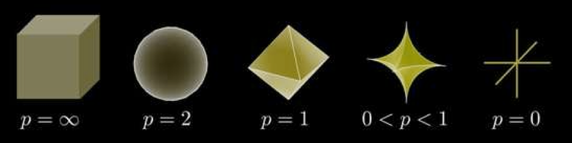
\includegraphics[width=1\linewidth]{figures/balls.png}
  \caption{$\ell_p$ unit ball for various values of $p$. The kinks
    in the cases $p \in \{1/2,1,\infty\}$ impose sparsity. Though the
  case $p = 1/2$ (and in fact any $p \in (0, 1)$) imposes sparsity,
it is non-convex...}
\end{figure}

\begin{marginfigure}[4cm]
  \centering
  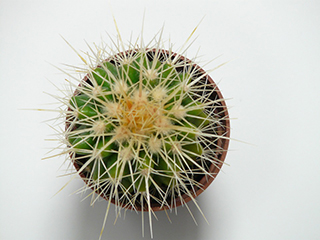
\includegraphics[width=1\linewidth]{figures/ball.jpg}
  \caption{$\ell_p$ ball with $0 < p \ll 1$.}
  \label{fig:flower}
\end{marginfigure}

\section{Preliminaries}
Sparsity and smoothness inducing priors can used to
perform jointly the prediction of a target variable and region
segmentation in multivariate analysis settings. Sparsity can be enforced by
penalizing the (sum of) absolute values of the regression coefficients, leading to the
so-called Lasso model. Smoothness can achieved in penalizing the spatial gradient of
the regression coefficients, to enforce smooth regions (``blobs'').
The Total-variation (TV)~\citep{rudin1992nonlinear,tibshirani2011solution} penalty has
proven to be particularly power for realizing such effects. Laplacian regularization
is an easier means to this end (because in leads to a differentiable problem),
but has weaker mini-max rates, and the visual effect is less appealing.

In the context of neuro-imaging, sparsity and smoothness have been compiled to yield
regression coefficients which are faithful to known neurobiological organization of the brain.
Specifically, it has been shown that one can employ priors like TV-$\ell_1$
 \citep{baldassarre2012,gramfort2013}, TV-ElasticNet \citep{dubois2014predictive},
and GraphNet  \citep{grosenick2013}
(aka Smooth-Lasso   \citep{hebiri2011})
%\footnote{Henceforth, we will use GraphNet and S-Lasso
%interchangeably.}
to regularize regression and classification
problems in brain imaging. Sparsity and smoo

We denote by ${\y} \in \mathbb{R}^{n}$ the targets to
be predicted (age, sex, IQ, etc.); the \textit{design matrix}
${\X}\in\mathbb{R}^{n \times p}$ are the masked (see Fig. \ref{fig:masking})
brain images related to the presentation of different
stimuli, or other brain acquisition (e.g gray-matter concentration
maps from anatomy, etc.). The integer $p$ is the number of voxels,
and $n$ the number of samples (images). In brain imaging, $n \ll p$;
typically, $p \sim 10^3-10^6$ (in full-brain analysis),
while $n \sim 10-10^3$ ($n$ being limited by the cost of acquisition,
etc.). $\nabla_x$ will denote the discrete spatial gradient operator
along the $x$-axis, $\nabla_y$ along the $y$-axis, etc.

%% Let $\mathcal P \subset \mathbb{R}^3$ be
%% the 3D image domain representing the region occupied by the brain --or
%% ROI (region of interest) thereof-- under  study, discretized regularly
%% on a finite grid.

  \begin{figure}[!htb] 
  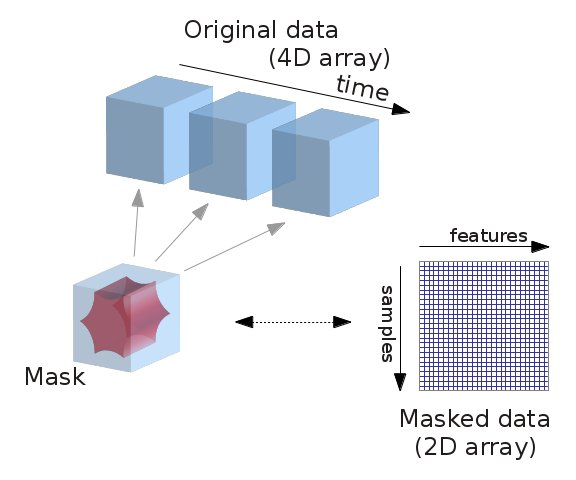
\includegraphics[width=1\linewidth]{figures/masking.jpg}
  \caption{\textbf{Masking} of volumic brain data (4D = 3D space + 1 time or samples)
    to produce a design matrix required in standard machine learning (clustering, classification, regression, etc.). For each 3D volume is a sample point. The values of the voxels in this volume which lie in the mask are collected into a feature vector. All these vectors are vertically stacked to produce an $n$-by-$p$ design matrix $\X$, where $p$ is the number of voxels in the mask. The mask can be just the region of the 3D cube occupied by the brain, or a subset of such. In the latter case, this typically corresponds to Region-of-Interests (ROIs) deemed to be interesting for an experiment. The former case is referred to as ``full brain'', and the mask typically contains $p = $ millions of voxels. See  \citep{abraham2014machine} for more details.}
  \label{fig:masking}
\end{figure}

\section{SpaceNet: sparse structured models for brain data}
Over time, a number of spatially regularized linear models have been proposed. These are mainly: Total-Variation (TV)
    \citep{michel2011tv}, TV-$\ell_1$   \citep{baldassarre2012,gramfort2013}, GraphNet   \citep{grosenick2013,hebiri2011},
  TV-ElasticNet   \citep{dubois2014predictive}, Sparse Variation   \citep{eickenberg2015total}, and social-sparsity   \citep{kowalski2013social}. These can all be written in a general framework as follows


\begin{equation}
  \underset{\w \in \mathbb R^p}{\text{minimize }}E(\w) := \ell(\y,\X\w) + \alpha \mathcal P(\w).
    \label{eq:opt_pb}
\end{equation}
The coefficients ${\w}$ define a spatial map in over the brain (one value per voxel).
The term {$\ell(\y,\X\w)$} is the
  {loss / data-fit term}. Popular choices include:
  $$
  \ell(\y,\X\w) = \frac{1}{n}\sum_{i=1}^n\begin{cases}\frac{1}{2}(\B{X}^T_i\w - y_i)^2,
    &\mbox{ \text{ for least-squares}}\\
    \log(1+\exp(-y_i\X_i^T\w)),
    &\mbox{ \text{ for logistic regression}},\\
    (1 - y_i\X^T_i\w)_+,&\mbox{\text{ for hinge loss (used in SVMs)}}\\
      \vdots\end{cases}
    $$
$\mathcal P(\w)$ is the penalty term, which simultaneously imposes both sparsity and structure (blobs). The different spatial regularization
methods that have appeared in neuro-imaging literature can be cast into this
correspond to different choices of the convex penalty $\mathcal P$ acting on the extended gradient of the coefficients $\w$. Viz,

\begin{equation}
  \begin{split}
  \mathcal P_\rho(\w) = \Omega(\nabla_\rho \w) := \begin{cases}
    \rho\|\w\|_1 + \frac{1}{2}(1-\rho)\|\nabla \w\|_{\text{Fro}}^2 = \sum_{j \in [\![p]\!]}\rho|w_j| + \frac{1}{2}(1-\rho)\|(\nabla \w)_j\|_2^2, &\mbox{ GraphNet
      %~\citep{grosenick2013,hebiri2011}
    },\\
    \|\nabla_\rho \w\|_{1+2,1} = \rho\|\w\|_1 + \|\nabla \w\|_{2,1} = \sum_{j  \in [\![p]\!]}\rho|w_j| + (1-\rho)\|(\nabla \w)_j\|_2, &\mbox{ for isotropic TV-$\ell_1$
      %~\citep{baldassarre2012,gramfort2013}
    },\\
    \|\nabla_\rho \w\|_{1,1} = \rho\|\w\|_1 + \|\nabla \w\|_{1,1} = \sum_{j  \in [\![p]\!]}\rho|w_j| + (1-\rho)\|(\nabla \w)_j\|_1, &\mbox{ for anisotropic TV-$\ell_1$
    },\\
    \|\nabla_\rho \w\|_{2,1} = \sum_{j  \in [\![p]\!]}\|(\nabla_\rho \w)_j\|_2, &\mbox{ for Sparse Variation
      % \citep{eickenberg2015total}
    },\\
      \vdots
    \end{cases}
  \end{split}
  \label{eq:penalty}
\end{equation}
where $\alpha > 0$ is a regularization parameter controls the total amount of regularization, and
$\rho$ ($0 < \rho \le 1$) is a mixing constant between
  the {sparsity-inducing} $\ell_1$ part and the
  {cluster-promoting} part of the penalty term.
  The particular case {$\rho = 1$} corresponds to the usual Lasso. Vanilla TV   \citep{michel2011tv} corresponds to TV-$\ell_1$ with $\rho = 0$.
 The matrix $\nabla_\rho$ is the extended discrete gradient operator defined in Chapter ~\ref{sec:notations}.  
\begin{marginfigure}[4cm]
  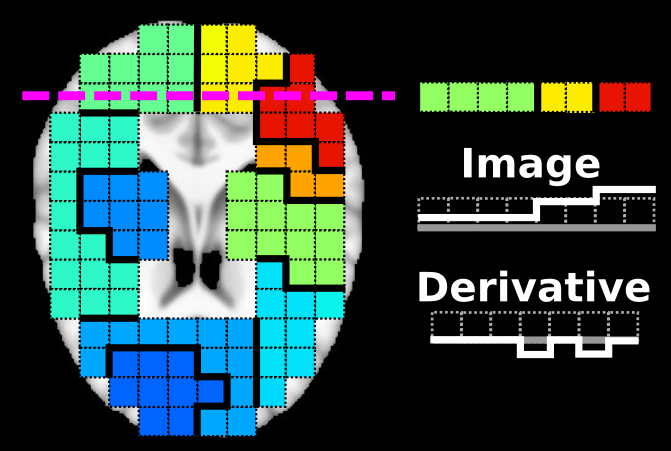
\includegraphics[width=1\linewidth]{figures/tv_cartoon_horizontal.png}
  \caption{A cartoon showing a sparse and blobby (step-wise constant / cartoon-like) brain map,
  as would be sought for by Total-Variation regularization \eqref{eq:ss}...}
  \label{fig:roi}
\end{marginfigure}
In the case of GraphNet \citep{grosenick2013,hebiri2011}, the penalties $\mathcal P(\w)$ in \eqref{eq:opt_pb} admit a Bayesian interpretation as a prior on the distribution of the coefficients $\w$
\begin{equation}
  \label{eq:bayesian}
p_{\alpha,\rho}(\w) \propto \prod_{j=1}^p\exp(-\alpha\rho |w_j|)\prod_{j=1}^p\exp\left(-\alpha(1-\rho)\sum_{l \sim \text{neigh}(j)}w_j\Delta_{j,l}w_l\right).
\end{equation}

The result of such regularized models, dubbed \emph{SpaceNet}
~\citep{spacenetohbm}, are brain maps which are both
sparse (i.e regression coefficients $\w$ are zero everywhere, except at
predictive voxels) and structured (blobby). See Fig. \ref{fig:roi}. The superiority of such
methods over methods without structured priors like the Lasso, ANOVA,
Ridge, SVM, etc. for yielding more intepretable maps and improved
prediction scores is now well established. See for example
  \citep{baldassarre2012,gramfort2013}. These priors are fast becoming
popular for brain decoding and segmentation. Indeed, they leverage a
feature-selection function
(since they limit the number of active voxels),
and also a structuring function
(since they penalize local
differences in the values of the brain map). For example, see Fig.
\ref{fig:spacenet_maps}.
Also, such priors produce state-of-the-art methods for automatic
extraction of functional brain atlases   \citep{abraham2013}.

\begin{mdframed}
  \paragraph{Submodular interpretation of TV.} We note anisotropic TV penalty on
  an arbitrary (undirected) graph $G = (V,E)$ is the \textit{Lovasz extension} of the \textit{cut-function}
  $F : 2^V \rightarrow \mathbb N$, $S \mapsto "\text{number of edges between } S \text{ and }V\setminus S"$,
defined by $F^L(x) := \mathbb E_{\lambda \sim \mathcal U([0,1])}[F(\{v \in V|x_v \ge \lambda\})]$, for all $x \in [0,1]^{\#V}$.
\end{mdframed}

\begin{figure}[!htbp]
  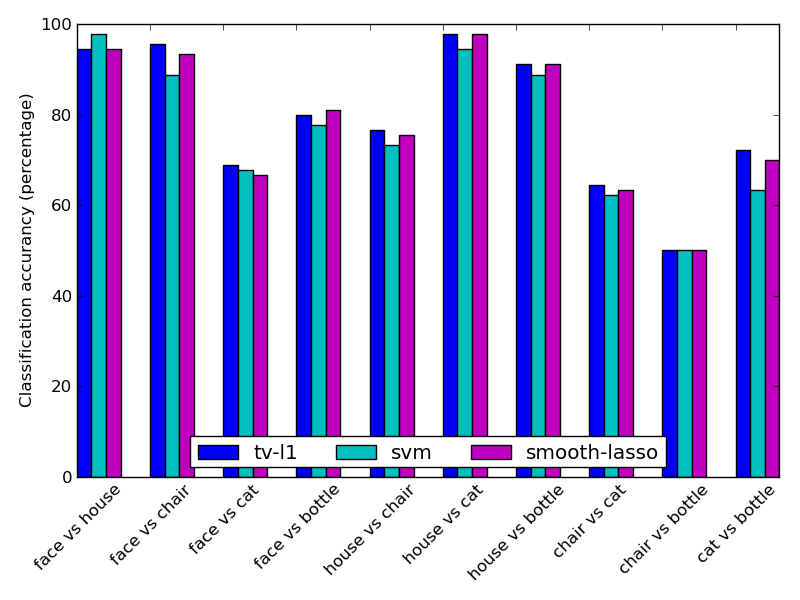
\includegraphics[width=1\linewidth]{figures/haxby_barchart.png}
  \caption{Bar chart showing percentage classification on leftout, for one-vrs-one classification on the visual recognition dataset~\citep{haxby2001}.
  }
  \label{fig:spacenet_bars}
\end{figure}

\section{Methods}
The SpaceNet model leads to difficult non-smooth mathematical optimization problems making their implementation and practical usability challenging. \citep{dohmatob2014benchmarking} benchmarked a rich variety of cutting-edge solvers for such problems, and gave crucial recommendations on how to effectively implement these algorithms in practice. In these benchmarks, the FISTA algorithm emerged as the go-to algorithm for the TV-L1 problem~\citep{dohmatob2015speeding}. These hints have been carefully used in implementing SpaceNet. Also as a preprocessing step, we use univariate feature-screening (ANOVA) to eliminate voxels which are irrelevant to the learning problem, thus reducing the size of the problem. As a result the implementation of SpaceNet is fast, robust, and automatically sets its parameters (internal cross-validation). All these technical details will be properly presented in the next few chapters.

\section{Experiments and results}
Here, we present results of experiments on publicly available fMRI datasets. The parameters of all the models were set by 8-fold cross-validation.

\paragraph{Classification.}
We compared SpaceNet (TV-L1 and Smooth-Lasso priors) with an SVM (Support Vector Machine) on the visual-recognition dataset~\citep{haxby2001}. This dataset consists of 6 subjects with 12 runs per subject. In each run, the subjects passively viewed images of eight object categories, grouped in 24-second blocks separated by intermittent rest periods. This experiment is a classification task: predicting the object category. The design matrix is made of time-series from the full-brain mask of $p=23,707$ voxels over 216 TRs (Repetition Times), of a single subject (subj1). 126 TRs were used for training all the models, whilst testing was done on 90 left-out TRs. The results are depicted in Figures 1 (bar chat) and 2 (brain maps).

\paragraph{Regression.}
Our second benchmark dataset is a study in which subjects were presented with mixed (gain/loss) gambles, and decided whether they would accept each gamble~\citep{jimura2012}. No outcomes of these gambles were presented during scanning, but after the scan three gambles were selected at random and played for real money. The prediction task here is to predict the magnitude of the gain and thus a regression on a continuous variable. The data is pooled across subjects, resulting in 768 samples, each an image of $p=33,177$ voxels. The results are shown in Figure 3.


\begin{marginfigure}%[!htb] 
  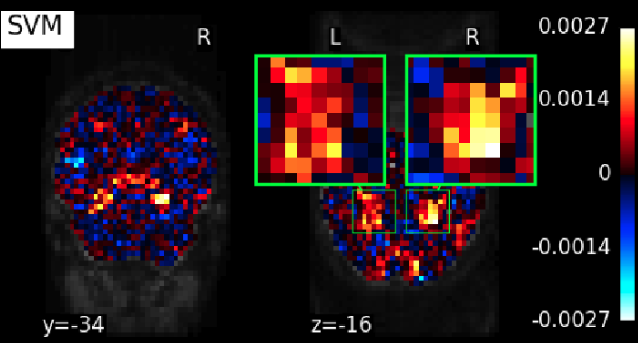
\includegraphics[width=1\linewidth]{figures/svm.png}
  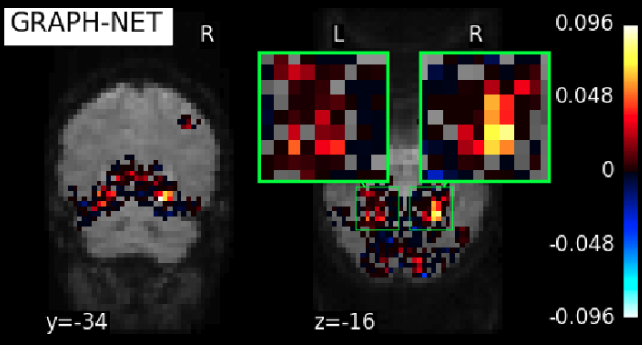
\includegraphics[width=1\linewidth]{figures/graphnet.png}
  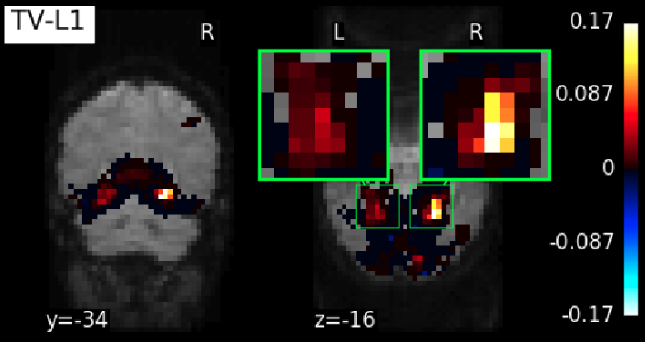
\includegraphics[width=1\linewidth]{figures/tvl1.png}  
  \caption{The figure shows results of comparing the SpaceNet  models TV-$\ell_1$ and
    Graph-Net against an SVM (Support Vector Machine) classifier on
    the visual-recognition dataset   \citep{haxby2001}
    As can be seen from the figure, SpaceNet priors (TV-$\ell_1$, GraphNet, etc.)
    yield stable and more intepretable maps. Figure taken from OHBM
    presentation   \citep{spacenetohbm}.}
  \label{fig:spacenet_maps}
\end{marginfigure}

\section{Conclusion}
We have presented SpaceNet, a family of priors for brain decoding which enforce both sparsity and structure, leading to better prediction scores and interpretable brain maps. We believe that such priors will become commonplace in future.

In the next chapter we open the ``black box'' and develop from ground-up, the details of such models, including their practical implementation on a computer.

% \clearpage
\bibliographystyle{plainnat}
\bibliography{bib_all}
